\documentclass[12pt,a4paper]{article}
\usepackage{fullpage}
\usepackage[top=2cm, bottom=4.5cm, left=2.5cm, right=2.5cm]{geometry}
\usepackage{amsmath,amsthm,amsfonts,amssymb,amscd}
\usepackage{lastpage}
\usepackage{enumerate}
\usepackage{fancyhdr}
\usepackage{mathrsfs}
\usepackage{xcolor}
\usepackage{graphicx}
\usepackage{listings}
\usepackage{hyperref}
\usepackage{txfonts}
\usepackage{titlesec}
\usepackage{esint}

\hypersetup{%
  colorlinks=true,
  linkcolor=blue,
  linkbordercolor={0 0 1}
}


\newcommand\course{8.03x - Vibrations and Waves}
\newcommand\hwnumber{1}               
\newcommand\MyName{Syed Suhaib Ahmad}
 
\renewcommand\lstlistingname{Algorithm}
\renewcommand\lstlistlistingname{Algorithms}
\def\lstlistingautorefname{Alg.}

\setlength{\parindent}{0.0in}
\setlength{\parskip}{0.05in}



\pagestyle{fancyplain}
\headheight 35pt
\lhead{\course}
\chead{\large\textbf{Problem Set 7}}
\rhead{\MyName{}}
\lfoot{}
\cfoot{\small\thepage}
\rfoot{}
\headsep 1.5em

\begin{document}

\subsubsection*{Problem 7.1 - Polarized radiation}
Write down the electric field and associated magnetic field in vacuum for traveling plane waves. The amplitude of the electric vector is $E_0$ and the frequency is $\omega$.
\begin{enumerate}
    \item[(a)]The radiation is linearly polarized in the $y-z$ plane at an angle of 45° with the $y-$axis, and it is traveling in the $+x$ direction. There are two solutions.
    \item[(b)]The radiation is circularly polarized in the $y-z$ plane, and it is traveling in the $+x$ direction. There are two solutions.
\end{enumerate}
\textbf{Solution(a)}
\\
\\There are two solutions since the electric field vector can be at an angle of $\pm$45° with respect to the $y-$axis.
\begin{equation}
\begin{aligned}
    \boldsymbol{\Vec{E}} &= E_0\cos(kx-\omega t)\left(\sin\left(\frac{\pi}{4}\right)\boldsymbol{\hat{y}} \pm \cos\left(\frac{\pi}{4}\right)\boldsymbol{\hat{z}}\right), \\
    \boldsymbol{\Vec{B}} &= \frac{E_0}{c}\cos(kx-\omega t)\left(\boldsymbol{\hat{x}}\times\left(\sin\left(\frac{\pi}{4}\right)\boldsymbol{\hat{y}} \pm \cos\left(\frac{\pi}{4}\right)\boldsymbol{\hat{z}}\right)\right).
\end{aligned}
\end{equation}

Thus, the two electric field vectors along with their corresponding magnetic field vectors are
\begin{equation}
\begin{aligned}
    \boldsymbol{\Vec{E}}_{\pi/4} &= \frac{E_0}{\sqrt{2}}\cos(kx-\omega t)(\boldsymbol{\hat{y}}+\boldsymbol{\hat{z}}), 
    & \boldsymbol{\Vec{B}}_{\pi/4} &= \frac{E_0}{c\sqrt{2}}\cos(kx-\omega t)(\boldsymbol{\hat{z}}-\boldsymbol{\hat{y}}), \\
    \boldsymbol{\Vec{E}}_{-\pi/4} &= \frac{E_0}{\sqrt{2}}\cos(kx-\omega t)(\boldsymbol{\hat{y}}-\boldsymbol{\hat{z}}), 
    & \boldsymbol{\Vec{B}}_{-\pi/4} &= \frac{E_0}{c\sqrt{2}}\cos(kx-\omega t)(\boldsymbol{\hat{z}}+\boldsymbol{\hat{y}}).
\end{aligned}
\end{equation}
\textbf{Solution(b)}
\\
\\Circularly polarized radiation can be written as the sum of two orthogonal linearly polarized components with a phase difference of $\pm\pi/2$ radians.
\begin{equation}
    \begin{aligned}
        \boldsymbol{\Vec{E}}&=E_0\left(\cos(kx-\omega t)\boldsymbol{\hat{y}}\pm\sin(kx-\omega t)\boldsymbol{\hat{z}}\right), \\
        \boldsymbol{\Vec{B}}&=\frac{E_0}{c}\left(\cos(kx-\omega t)\boldsymbol{\hat{z}}\mp\sin(kx-\omega t)\boldsymbol{\hat{y}}\right).
    \end{aligned}
\end{equation}
Now, we have two solutions for the electric and magnetic field vectors; right-handed and left-handed circular polarization (RCP and LCP).
\\
\\RCP:
\begin{equation}
    \begin{aligned}
        \boldsymbol{\vec{E}}&=E_0\left(\cos(kx-\omega t)\boldsymbol{\hat{y}}+\sin(kx-\omega t)\boldsymbol{\hat{z}}\right), \\
        \boldsymbol{\vec{B}}&=\frac{E_0}{c}\left(\cos(kx-\omega t)\boldsymbol{\hat{z}}-\sin(kx-\omega t)\boldsymbol{\hat{y}}\right).
    \end{aligned}
\end{equation}
LCP:
\begin{equation}
    \begin{aligned}
        \boldsymbol{\vec{E}}&=E_0\left(\cos(kx-\omega t)\boldsymbol{\hat{y}}-\sin(kx-\omega t)\boldsymbol{\hat{z}}\right), \\
        \boldsymbol{\vec{B}}&=\frac{E_0}{c}\left(\cos(kx-\omega t)\boldsymbol{\hat{z}}+\sin(kx-\omega t)\boldsymbol{\hat{y}}\right).
    \end{aligned}
\end{equation}

\subsubsection*{Problem 7.2 - Radiation from an accelerated charge}
A charge, $q$, initially at rest, is given a brief acceleration along the $z$ axis. Let this occur at the origin of the coordinate system at $t=0$.
\begin{enumerate}
    \item[(a)]Give the arrival times, the relative strengths, and specify the directions of the radiated electric field seen by three observers in the $y-z$ plane at a large distance $R$ from the origin. One observer is on the $y-$axis, one on the $z-$axis, and one is on a radius making an angle of 30° to the $z-$axis.
    \item[(b)]Describe the orientation and magnitude of the associated radiated magnetic fields.
\end{enumerate}
\textbf{Solution(a)}
\\
\\The general formula for the radiated electric field is
\begin{equation}
    \boldsymbol{\vec{E}}_{\text{rad}}=-\frac{q\boldsymbol{\vec{a}}_{\perp}\left(t-\frac{R}{c}\right)}{4\pi\epsilon_0Rc^2}.
\end{equation}
Eq. (6) suggests that the radiated electric field is antiparallel to the orthogonal component of acceleration to the position vector between the initial position of charge and the observer. Arrival times in all cases is $R/c$. 
\\
\\Now, we apply the above relation to each case.
\begin{equation}
    \begin{aligned}
        \boldsymbol{\vec{E}}_{\theta=\pi/2}&=\frac{qa_{\perp}t'\sin\left(\frac{\pi}{2}\right)}{4\pi\epsilon_0Rc^2}(\boldsymbol{\hat{r}}_{\pi/2}\times\boldsymbol{\hat{x}})=-\frac{qa_{\perp}t'}{4\pi\epsilon_0Rc^2}\boldsymbol{\hat{z}}\\
        \boldsymbol{\vec{E}}_{\theta=\pi/6}&=\frac{qa_{\perp}t'\sin\left(\frac{\pi}{6}\right)}{4\pi\epsilon_0Rc^2}(\boldsymbol{\hat{r}}_{\pi/6}\times\boldsymbol{\hat{x}})=\frac{qa_{\perp}t'}{8\pi\epsilon_0Rc^2}\left(\frac{\sqrt{3}}{2}\boldsymbol{\hat{y}}-\frac{1}{2}\boldsymbol{\hat{z}}\right)\\
        \boldsymbol{\vec{E}}_{\theta=0}&=\frac{qa_{\perp}t'\sin(0)}{4\pi\epsilon_0Rc^2}(\boldsymbol{\hat{r}}_0\times\boldsymbol{\hat{x}})=0.
    \end{aligned}
\end{equation}
Given that $t'=t-R/c$ and $\boldsymbol{\hat{y}}\times\boldsymbol{\hat{z}}=\boldsymbol{\hat{x}}$, where $\boldsymbol{\hat{x}}$ is coming out of the plane of the page. We can see that the radiated electric field is maximum at right angles to the direction of acceleration.
\\
\\\textbf{Solution(b)}
\\
\\The magnetic field in all three cases is in the direction of the unit vector $-\boldsymbol{\hat{x}}$ (into the page). It still takes the same amount of time as the radiated electric field to arrive at the point of observation. The relative strength of the radiated magnetic fields is $|\,\boldsymbol{\vec{E}}_{\text{rad}\,}|/c$.
 
\subsubsection*{Problem 7.3 - Radiation from an accelerated charge}
A point charge $+q$ has been moving with constant velocity $w$ along a straight line until the time $t=t_0$. In the short time interval from $t=t_0$ to $t=t_0+\Delta t$, a force perpendicular to the trajectory changes the direction without changing the magnitude of the velocity. After the time $t=t_0+\Delta t$ the charge again moves with velocity $w$ along a straight line forming a small angle $\Delta\alpha$ with the initial trajectory.
\begin{figure}[h]
    \centering
    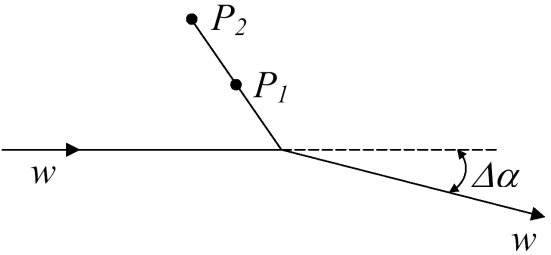
\includegraphics[width=0.6\linewidth]{figs/fig_prob_7.3.png}
   % \caption{Caption}
  %  \label{fig:enter-label}
\end{figure}
\begin{enumerate}
    \item[(a)]What is the direction of the electric field caused by the acceleration, at the distant point $P_1$?
    \item[(b)] In what direction is the radiation intensity of the accelerated charge most intense?
    \item[(c)]Where is it least intense?
    \item[(d)]Point $P_2$ is twice as far from the bend in the trajectory as $P_1$. By what fraction does the amplitude of the magnetic disturbance decrease as the radiation pulse moved from $P_1$ to $P_2$?
    \item[(e)]What is the total energy radiated?
\end{enumerate}
Make careful sketches in answering parts (a), (b), (c).
\\
\\\textbf{Solution(a)}
\\
\\Since $\Delta\alpha$ is small, we can assume that acceleration along the $x-$axis is negligible.
\[\boldsymbol{\vec{a}}=\frac{w\sin\Delta\alpha}{\Delta t}\boldsymbol{\hat{y}}\approx\frac{w\Delta\alpha}{\Delta t}\boldsymbol{\hat{y}}.\]
Thus, the component of this acceleration that is perpendicular to the position vector of $P_1$ is
\[a_{\perp}=\frac{w\Delta\alpha}{\Delta t}\sin\theta.\]
The radiated electric field at $P_1$ must be antiparallel to $a_{\perp}$. Hence, the electric field caused by the acceleration is given by
\[\boldsymbol{\vec{E}}=\frac{qa_{\perp}\sin\theta}{4\pi\epsilon_0Rc^2}(\boldsymbol{\hat{r}}_{P_1}\times\boldsymbol{\hat{z}})=\frac{qw\Delta\alpha\sin\theta}{4\pi\epsilon_0Rc^2}(\cos\theta\boldsymbol{\hat{x}}+\sin\theta\boldsymbol{\hat{y}}).\]
($\boldsymbol{\hat{x}}\times\boldsymbol{\hat{y}}=\boldsymbol{\hat{z}}$, where $\boldsymbol{\hat{z}}$ is out of the plane of the page).
\\
\\\textbf{Solution(b)}
\\
\\The intensity is most intense in the $x-z$ plane.
\\
\\\textbf{Solution(c)}
\\
\\Along the $y-$axis.
\\
\\\textbf{Solution(d)}
\\
\\We know that $\boldsymbol{\vec{B}}=\boldsymbol{\vec{E}}/c\propto1/R$, thus the magnetic disturbance decreases by a factor of two.
\\
\\\textbf{Solution(e)}
\\
\\Using the general formula for power radiated by an accelerated charge (Larmor formula), we have
\[\text{Energy}=P\Delta t=\frac{q^2a^2\Delta t}{6\pi\epsilon_0c^3}=\frac{q^2w^2}{6\pi\epsilon_0c^3}\left(\frac{\Delta\alpha}{\Delta t}\right)^2\Delta t.\]

\subsubsection*{Problem 7.4 - Speed checked by radar}
A radar beam ($\lambda=3\,$cm) is reflected off a car as shown in the figure (head-on reflection). The radar transmitter is \underline{not} moving. The reflected beam is again received by the police; the frequency $f'$ of this reflected signal is measured by a stationary receiver on the police car. From this the velocity $v$ of the car is calculated. All this is done in a “black-box” in less than a small fraction of a second! A digital display tells the police officer your speed nicely converted into miles/hour.
\begin{figure}[h]
    \centering
    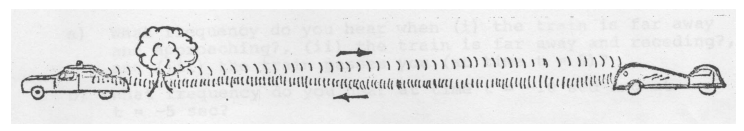
\includegraphics[width=1\linewidth]{figs/fig_prob_7.4.png}
    %\caption{Caption}
   % \label{fig:enter-label}
\end{figure}
\begin{enumerate}
    \item[(a)]What is the frequency of this radar transmitter?
    \item[(b)]Give an equation that relates $f$, $f'$ and $v$. (\textit{Hint: first calculate the frequency that the car “sees”, then send this signal back to the police.})
\end{enumerate}
\textbf{Solution(a)}
\\
\\The frequency can be easily calculated using
\[f=\frac{c}{\lambda}=\frac{3\times10^8}{3\times10^{-2}}=10^{10}\,\text{Hz}.\]
\textbf{Solution(b)}
\\
\\The Doppler shift equation for an electromagnetic wave is given by
\begin{equation}
    f_{\text{received}}=\left(\frac{1\pm\beta}{1\mp\beta}\right)f,
\end{equation}
where $\beta=v/c$. For the given scenario, the above equation can be approximated to
\[f_{\text{received}}\approx(1+\beta)f.\]
Thus, the frequency of reflected signal received by the police car is given by the expression
\[f'\approx(1+\beta)f_{\text{received}}\approx(1+\beta)^2f.\]


\subsubsection*{Problem 7.5 - Can’t you hear the whistle blowing?}
A train travels down a long straight track at a speed of 20\,m/sec ($\approx45$\,mph) blowing its whistle constantly ($f=1000$\,Hz). You, the observer, are standing at a point 100\,m from the track (see figure). Define time $t=0$ the moment that the train is closest to you.
\begin{figure}[h]
    \centering
    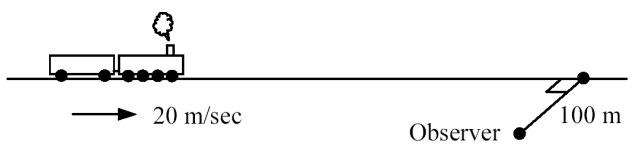
\includegraphics[width=0.9\linewidth]{figs/fig_prob_7.5.png}
    %\caption{Caption}
   % \label{fig:enter-label}
\end{figure}
\begin{enumerate}
    \item[(a)]What frequency do you hear when (i) the train is far away and approaching?, (ii) the train is far away and receding?, and (iii) the train passes you (at time $t=0$)?
    \item[(b)]What frequency do you hear at time $t=-10$\,sec and at $t=-5$\,sec?
    \item[(c)]Sketch the curve of the frequency that you hear versus time.
\end{enumerate}
\textbf{Solution(a)}
\\
\\Doppler effect effect equation for sound waves is
\begin{equation}
    f'=\left(\frac{v_{\text{S}}\pm v_{\text{O}}\cos\theta_O}{v_{S}\mp v_{\text{T}}\cos\theta_T}\right)f,
\end{equation}
where $v_{\text{S}}$, $v_{\text{O}}$, and $v_{\text{T}}$ are velocities of sound in air, observer, and transmitter respectively. In our case, $v_O=0$ and $v_T\ll v_S$ hence Eq. (9) can be simplified to 
\begin{equation}
    f'\approx\left(1+\frac{v_T}{v_S}\cos\theta_T\right)f.
\end{equation}
Thus, the frequencies are 
\[\text{(i)\,\,}\theta_T=0:\,f'\approx1059\,\text{Hz},\,\,\,\,\,\text{(ii)\,\,}\theta_T=\pi:\,f'\approx941\,\text{Hz},\]
\[\text{(iii)\,\,}\theta_T=\pi/2:\,f'\approx1000\,\text{Hz}.\]
\textbf{Solution(b)}
\[f'_{t=-10}\approx\left(1+\frac{v_T}{v_S}\frac{200}{\sqrt{200^2+100^2}}\right)f\approx1053\,\text{Hz}.\]
\[f'_{t=-5}\approx\left(1+\frac{v_T}{v_S}\frac{100}{\sqrt{100^2+100^2}}\right)f\approx1042\,\text{Hz}.\]
\textbf{Solution(c)}
\begin{figure}[h]
    \centering
    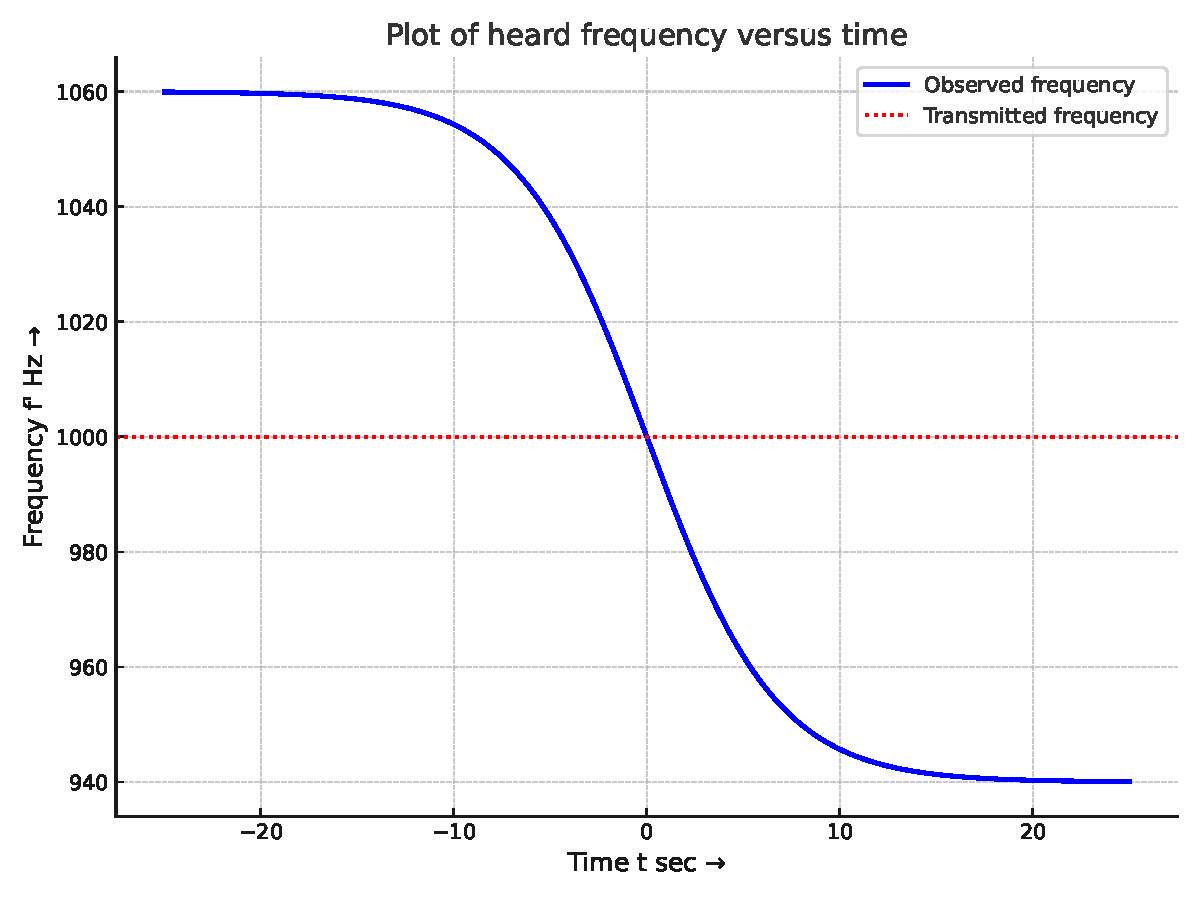
\includegraphics[width=1\linewidth]{figs/fig_sol_7.5c.pdf}
    %\caption{Caption}
    %\label{fig:enter-label}
\end{figure}

\subsubsection*{Problem 7.6 - Our expanding universe - simplified}
The figure below illustrates the famous expanding balloon analogy for our universe. All of space is represented by the surface of the spherical balloon, and clusters of galaxies are represented by spots
painted on this surface; the radius of the balloon corresponds to $R(t)$, the “radius” of the universe. As the balloon expands, the spots remain at constant angular separations ($\theta$) from one another. Let the balloon expand at a constant rate.
\begin{enumerate}
    \item[(a)]Prove that
    \begin{equation}
        \left(\frac{\Delta s}{\Delta t}\right)=\left(\frac{1}{R}\frac{\Delta R}{\Delta t}\right)\text{s}
    \end{equation}
\end{enumerate}
Here $s$ is the separation between any two spots (on the surface) and ($\Delta s/\Delta t$) is the speed of recession of one spot from another.
\\
\\Note that eq. (11) is equivalent to Hubble’s Law:
\begin{equation}
    v=Hr
\end{equation}
\begin{enumerate}
    \item[(b)]What is $H$ in terms of the symbols used in eq. (11)? Check that your answer is dimensionally correct; $H$ in general is expressed in km/sec per Mpc. 
\end{enumerate}
The light photons from distant galaxies may be represented by “ants” crawling along the balloons surface at speed $l$.
\begin{figure}[h]
    \centering
    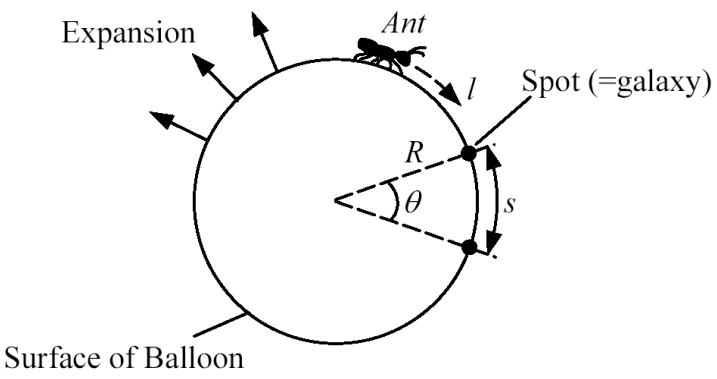
\includegraphics[width=0.7\linewidth]{figs/fig_prob_7.6.png}
   % \caption{Caption}
  %  \label{fig:enter-label}
\end{figure}
\begin{enumerate}
    \item[(c)]Show that for uniform cosmic expansion [i.e., $(\Delta R/\Delta t)=\text{constant}$] there is a distance (s) from beyond which these ants cannot ever reach our galaxy (this distance is called the horizon)! 
\end{enumerate}
\textbf{Let us now turn to the way we looked at our world a few years ago, before the discovery of “dark energy”. Dark energy is responsible for the fact that the expansion  of the universe, according to present believe, is accelerating, not decelerating. This mysterious dark energy is presently one of the “hottest” topics in all of physics. In what follows, pretend that there is no dark energy.}
\\
\\Consider an expanding (gravitating) gaseous sphere of uniform mass density $\rho$, with a total mass $M$ and a radius $R(t)$. A gas particle at the surface of this sphere will move radially outward with velocity $v$ so that
\begin{equation}
    \frac{v^2}{2}=\frac{GM}{R}+\text{constant}
\end{equation}
Here $v=\Delta R/\Delta t$ is the radial speed.
This must be a familiar equation from your 8.01 days. If the constant is positive then the expansion will never stop (too much kinetic energy); if the constant is negative then the expansion will ultimately stop and a collapse under the influence of gravitational forces will follow.
\begin{enumerate}
    \item[(d)]Show that eq. (13) can be written in the form:
    \begin{equation}
        \left(\frac{1}{R}\frac{\Delta R}{\Delta t}\right)^2=\frac{8\pi G\rho}{3}+\frac{2(\text{constant})}{R^2}
    \end{equation}
\end{enumerate}
In the following we will introduce a subscript 0 when we refer to our present time.
\\
\\In the following assume $H_0=70\,\frac{\text{km/sec}}{\text{Mpc}}$ and $G=6.7\times10^{-11}$ (SI unit).
\begin{enumerate}
    \item[(e)]What is the minimum required density of our universe now ($\rho_0$) to make it closed? 
\end{enumerate}
Replace in eq. (14) $\rho$ by $\frac{M}{\frac{4}{3}\pi R^2}$. Here $M$ is the total mass of the universe.
\begin{enumerate}
    \item[(f)]Show that in case of a flat universe the radius of the universe $R(t)\propto t^{2/3}$. 
\end{enumerate}
From this it follows immediately that $H=\frac{2}{3t}$ (show that) and consequently the age of our universe 2 now $t_0=\frac{2}{3H_0}\approx9.3\times10^9$\,years.
\begin{enumerate}
    \item[(g)]Your modified eq. (14) relates $H^2=\left(\frac{1}{R}\frac{\Delta R}{\Delta t}\right)^2$ with $R$. Show that Hubble’s constant must have been larger in the past.
    \item[(h)]Could $H$ become negative? What consequence would that have for our “red-shifted” galaxies.
\end{enumerate}
\textbf{Solution(a)}
\\
\\As angular separation is constant and $\theta=s/R$, any change in $s$ and a corresponding change in $R$ should not affect $\theta$.
\[\frac{s}{R}=\frac{s+\Delta s}{R+\Delta R}\Rightarrow sR+s\Delta R=sR+\Delta sR.\]
Dividing throughout by $\Delta t$ gives
\[\frac{\Delta sR}{\Delta t}=\frac{s\Delta R}{\Delta t}\Rightarrow\left(\frac{\Delta s}{\Delta t}\right)=\left(\frac{1}{R}\frac{\Delta R}{\Delta t}\right)s.\]
\textbf{Solution(b)}
\\
\\Hubble's law suggests that the recession velocity, $v$, is directly proportional to the distance $d$ between the two objects (earth and galaxies in general), where $H$ is the proportionality constant (units of 1/second). In the analogy described in the problem, we have a very similar relation where $\Delta s/\Delta t=v$, $s=d$, and $1/R(\Delta R/\Delta t)=H$. $\Delta R/\Delta t$ and $1/R$ have units of meter / second and 1 / meter, respectively. Thus, their product has units of 1 / second (same as $H$).
\\
\\\textbf{Solution(c)}
\\
\\If the maximum velocity of the ants is equal to the recession velocity $(l=\Delta s/\Delta t)$ and the cosmic expansion is constant $(k=\Delta R/\Delta t)$, the ants will never reach the observer galaxy. 
\[l=\frac{k}{R}s_{\text{max}}\Rightarrow s_{\text{max}}=\frac{Rl}{k}.\]
\textbf{Solution(d)}
\\
\\Multiplying Eq. (13) with $2/R^2$ gives
\begin{equation}
    \frac{v^2}{R^2}=\frac{2GM}{R^3}+\frac{2(\text{constant})}{R^2}.
\end{equation}
Now we introduce the following quantities into Eq. (15):
\[v=\frac{\Delta R}{\Delta t}\,\,\,\,\,\text{and}\,\,\,\,\,\rho=\frac{M}{\frac{4}{3}\pi R^3}=\frac{3M}{4\pi R^3}.\]
Eq. (15) now becomes
\[\frac{1}{R^2}\left(\frac{\Delta R}{\Delta t}\right)^2=\frac{4\pi}{3}\times\rho\times2G+\frac{2(\text{constant})}{R^2}\]
\[\left(\frac{1}{R}\frac{\Delta R}{\Delta t}\right)^2=\frac{8\pi G\rho}{3}+\frac{2(\text{constant})}{R^2}\]
\textbf{Solution(e)}
\\
\\For a flat universe, constant $=0$. From part b, $H=1/R(\Delta R/\Delta t)$. The result from part d can now be written as
\[H^2=\frac{8\pi G\rho}{3}\Rightarrow\rho_0=\frac{3H_0^2}{8\pi G}\approx10^{-26}\,\text{kg\,m}^{-3}.\]
\textbf{Solution(f)}
\\
\\As we are still considering a flat universe, constant $=0$. Eq. (15) gives 
\[\left(\frac{1}{R^2}\frac{\Delta R}{\Delta t}\right)^2=\frac{2GM}{R^3}\Rightarrow t=\int\sqrt{R/2GM}\,dR\Rightarrow t=\frac{2R^{3/2}}{3\sqrt{2GM}}.\]
The above result clearly shows that $R\propto t^{2/3}$. 
\\
\\Let $R=ct^{2/3}$ and $\Delta R/\Delta t=2/3(ct^{-1/3})$. We know that $H=1/R(\Delta R/\Delta t)$. 
\[H=\frac{1}{ct^{2/3}}\times\frac{2}{3}ct^{-1/3}=\frac{2}{3t}.\]
Finally, the age of the universe using the model we have assumed so far is
\[t_0=2/3H_0\approx9.3\times10^9\,\text{years}.\]
\textbf{Solution(g)}
\\
\\Combining $t\propto R^{3/2}$ and $H=2/3t$ gives
\[H\propto\frac{1}{R^{3/2}}.\]
Since the radius of the universe $R$ (radius of the ballon in our case) was smaller in the past, $H$ must have been larger.
\\
\\\textbf{Solution(h)}
\\
\\If $H$ becomes negative, $\Delta R/\Delta t$ also becomes negative, which would imply that universe is collapsing and all objects are coming closer relative to each other. This would change all the redshift observations to blueshift!

\end{document}